\chapter{Introducción}\label{ch:introduccion}

La habilidad del ser humano para navegar en entornos desconocidos se fundamenta en su capacidad para identificar patrones comunes entre diversas estancias.
Esto le permite, mediante un proceso de exploración, localizar su objetivo en un espacio nunca antes visitado.

Esta capacidad para recorrer entornos desconocidos ha demostrado ser de gran interés para su integración en plataformas robóticas reales, debido a su versatilidad tanto funcional como comercial.
Históricamente, en el ámbito de la robótica, la navegación ha estado estrechamente vinculada a la sensorización y al uso de tecnologías como \ac{LiDAR}, empleando técnicas como \ac{SLAM}.
No obstante, estas aproximaciones presentan limitaciones a la hora de generalizar el problema de la navegación en entornos no explorados, además de mayores desafíos en escenarios abiertos o simétricos.

Como alternativa, actualmente se aborda este reto mediante el uso de redes neuronales entrenadas con diversos algoritmos de \textit{Deep Learning}.
Es lo que se conoce como las soluciones de navegación basadas en aprendizaje, que emplean, principalmente, sensores visuales.
Es por ello, que el problema recibe el nombre de Navegación Visual Semántica.
Algunos de los trabajos más recientes en esta dirección son los siguientes\citep{ramrakhya2023,zhang2022,Huang2023}.

El entrenamiento de estas soluciones se lleva a cabo en entornos virtuales, donde un agente tiene la capacidad de desplazarse por espacios reales renderizados.
Esta metodología permite acelerar el proceso de aprendizaje al aprovechar máquinas especializadas en computación paralela, y algoritmos diversos como el aprendizaje por refuerzo o el aprendizaje por imitación.

Con el fin de demostrar y comparar la capacidad de navegación de estos agentes, se les asigna la tarea de localizar un objeto dentro de estancias renderizadas, las cuales no han explorado previamente.

Se ha demostrado que estos agentes son capaces de alcanzar altos porcentajes de éxito en la consecución de sus objetivos dentro de entornos virtuales.
No obstante, cuando se implementan estas redes en el mundo real, surgen desafíos relacionados con la \textit{\textbf{adaptación de dominio}}.
Estos problemas se deben, en parte, a la menor precisión de los sensores y a factores inherentes al entorno físico, como variaciones en la iluminación.

El propósito de estas redes neuronales es emular el comportamiento humano, lo cual explica que las entradas a las redes correspondan habitualmente a los mismos estímulos sensoriales que utilizan los seres humanos.
Por esta razón, se emplean de manera predominante imágenes RGB, odometría y cámaras de profundidad.
Sin embargo, el ser humano no se desplaza únicamente en función de las imágenes que percibe, sino que también otorga un sentido semántico a los objetos dentro de esas imágenes.
De este modo, es capaz de identificar rápidamente la función de cada elemento que observa, como suelos, paredes, armarios o sillas, asignándoles una categoría semántica de manera casi instantánea.

Esta capacidad para categorizar visualmente ha sido abordada con gran éxito en el campo de la visión artificial.
En la actualidad, contamos con segmentadores semánticos que han demostrado un rendimiento sobresaliente\cite{Seichter2020EfficientRS}.

En este proyecto, pretendemos estudiar el impacto que los sensores de segmentación semántica tienen en los modelos de navegación visual semántica.
Postulamos que son una fuente de información que puede aliviar el problema de la adaptación de dominio, y, por lo tanto, el desarrollo de modelos de navegación que puedan funcionar en el mundo real, y no solo en entornos virtuales.

Así, en este trabajo, proponemos desarrollar soluciones de navegación visual semántica empleando aprendizaje por imitación (\textbf{IL} (Imitation Learning)) que recibirán imágenes de segmentación semántica como entrada.
Posteriormente, se comparará su rendimiento con respecto a modelos que utilizan imágenes RGB, tanto en entornos virtuales como en escenarios del mundo real.

En la figura\ref{fig:semnav} proponemos una representación del tipo de soluciones que se van a desarrollar, denominadas como SemNav, puede observarse como a la entrada de la red se ingresará información de segmentación semántica, complementada con otro tipo de información, que ayudará al modelo a completar la navegación en entornos desconocidos.

\begin{figure}
    \centering
    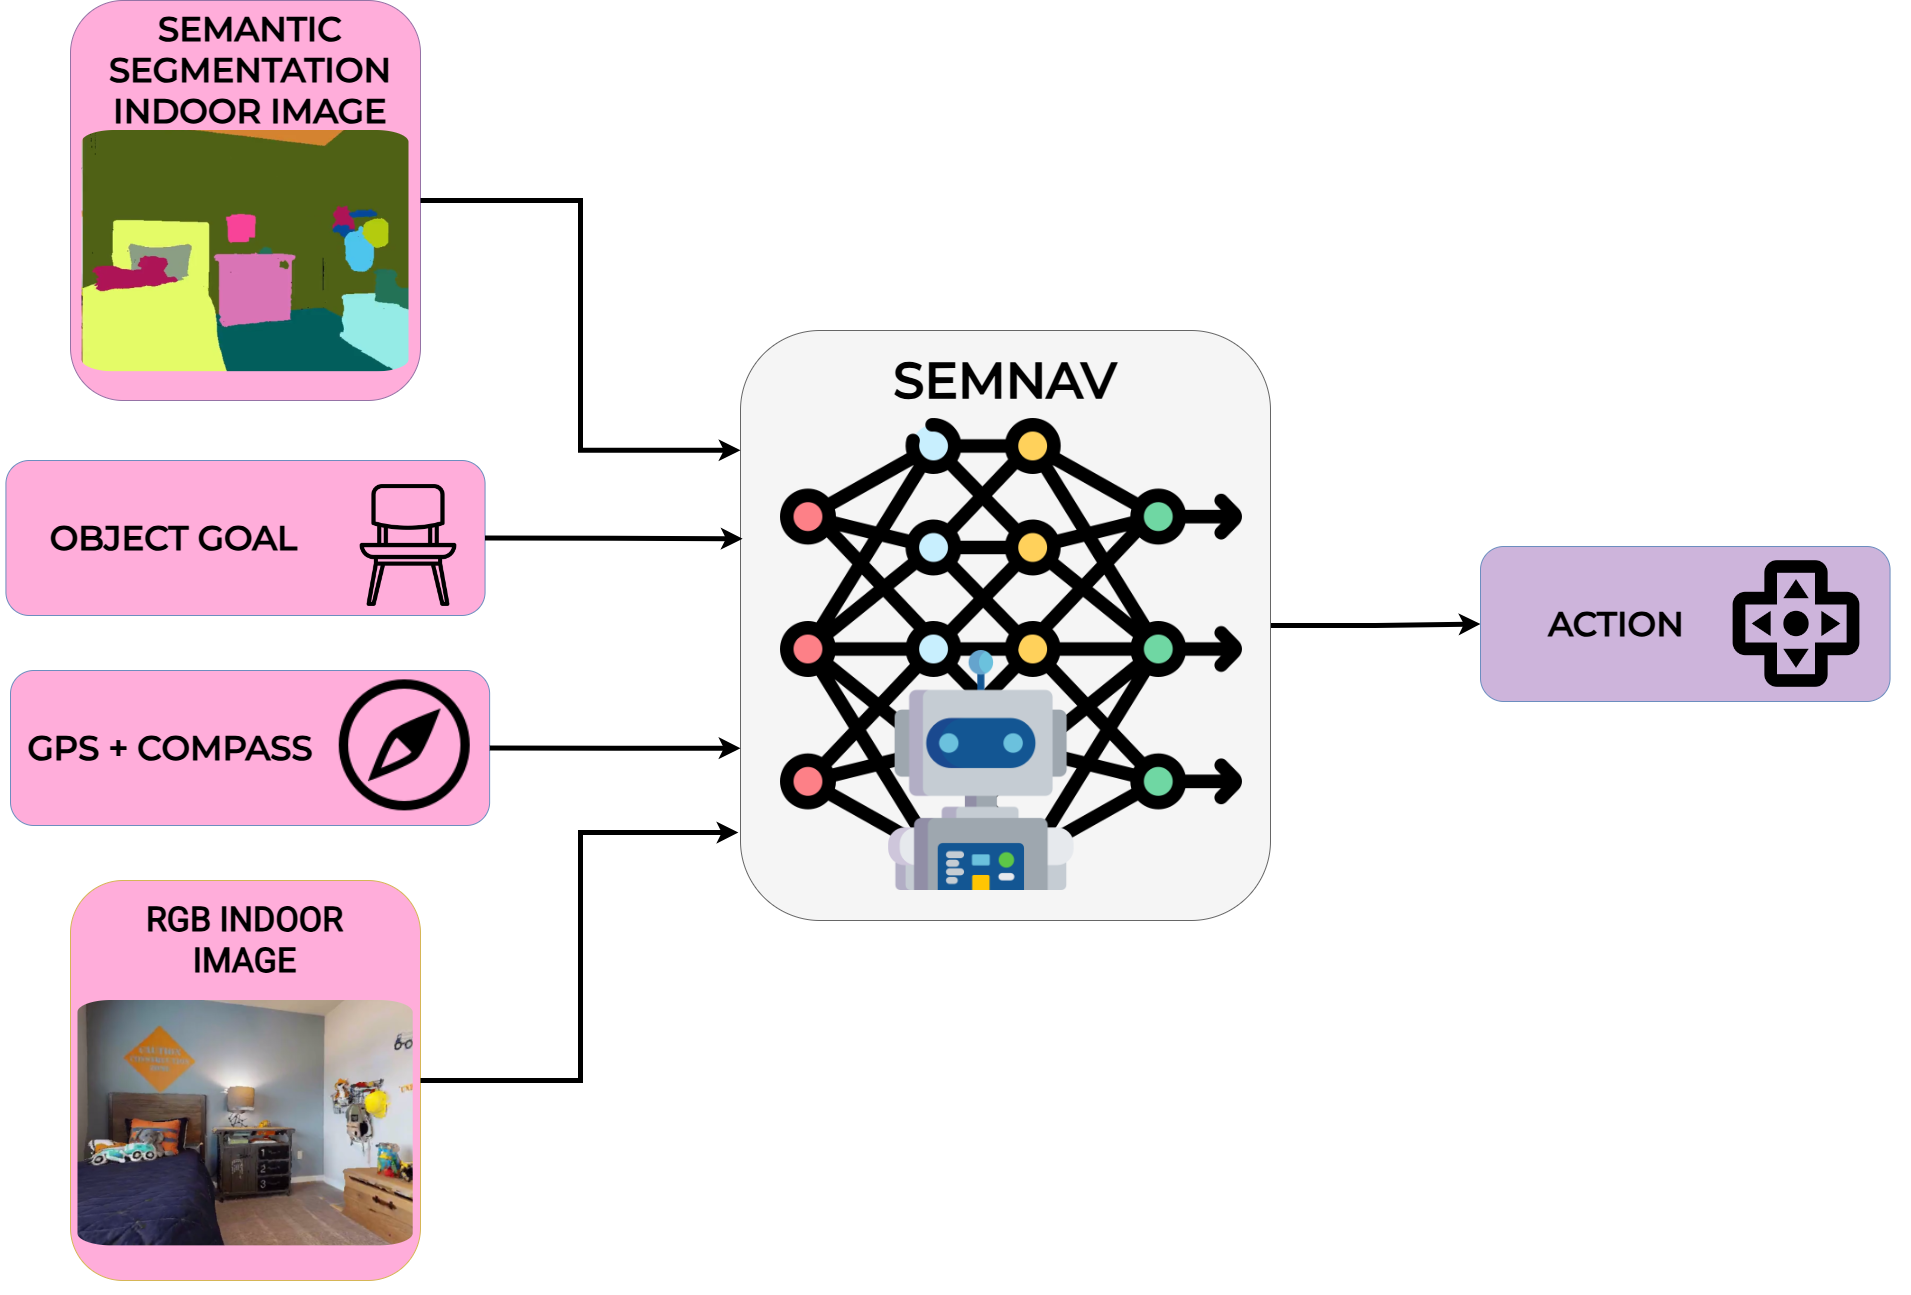
\includegraphics[width=\textwidth]{figuras/semnav_model}
    \caption{Modelo SEMNav para la navegación basada en información de segmentación semántica del entorno.}
    \label{fig:semnav}
\end{figure}